\subsection{RMW Layer APIs}
% - NOTE: -------------------------------------------------------------
\subsubsection{INIT: rmw\_init.c}
\todo{HERE!!!!!}


% - NOTE: -------------------------------------------------------------
\subsubsection{WORKING: wait.h}

\textbf{1. \apiarg{rmw\_wait}{  rmw\_subscriptions\_t * subscriptions,
rmw\_guard\_conditions\_t * guard\_conditions,
rmw\_services\_t * services,
rmw\_clients\_t * clients,
rmw\_events\_t * events,
rmw\_wait\_set\_t * wait\_set,
const rmw\_time\_t * wait\_timeout}}: Waits on sets of different entities and returns when one is ready. This function adds middleware-specific conditions to the wait set and waits until one or more become ready, or until the timeout is reached. \footnote{Elapsed time is measured against the system clock. Timeout granularity is thus bound to that of the aforementioned clock and, depending on the underlying implementation, to that of platform-specific APIs to sleep and/or wait. \textbf{The amount of time this function actually waits may be either above or below the specified timeout.}} Called API \api{uxr\_run\_session\_until\_data~()} in XRCE-DDS layer.
\begin{figure}[htbp!]
    \centering
    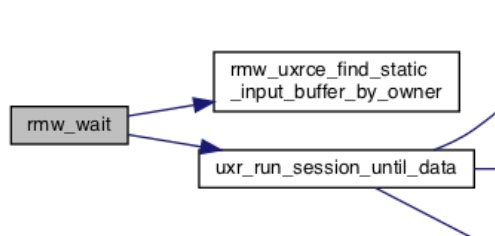
\includegraphics[width=0.5\linewidth]{Sec/Implementation/rmw/fig/rmw_wait().jpg}
    \caption{Function code: rmw\_wait()}
    \vspace{-0.1in}
\end{figure}